\section{Evaluation} \label{sect:eval}

\subsection{Methodology} \label{sect:methodology}
{\bf Model and dataset.} We target TinyAgent~\cite{tinyagent}, an open-source, on-device agent framework for macOS built on LLMCompiler~\cite{llmcompiler}. Our experiments use TinyAgent-7B~\cite{tinyagent_7b} as the backend LLM, a fine-tuned variant of WizardLM-2-7B~\cite{wizardlm2}. TinyAgent’s fine-tuning dataset~\cite{tinyagent_dataset} serves three roles: \prefill uses the training split for tool clustering and combination selection, and the test split is used for evaluation. Before each task, we flush the system’s page cache to isolate the cost of loading the KV cache from storage.


{\bf Hardware and software.} Experiments run on an Apple Mac mini with an M4 Pro chip~\cite{apple_m4_pro_max}, 64 GB of memory, 512 GB of SSD storage, 12 CPU cores, and 16 GPU cores. We build \prefill and \decode on MLX-LM~\cite{mlx_lm} and MLX-engine~\cite{mlx_engine}. MLX-LM is Apple Silicon’s official LLM inference package, backed by MLX~\cite{mlx}. MLX-engine is an open-source MLX LLM engine from LM Studio. The software stack comprises MLX v0.25.2, a modified MLX-LM v0.25.1, and MLX-engine commit \#ecc2cf4 on macOS Sequoia 15.5.


\subsection{\prefill} \label{sect:eval_prefill}

{\bf Planner accuracy.}
In line with prior work~\cite{llmcompiler,tinyagent}, we define the Planner accuracy by constructing a Directed Acyclic Graph (DAG) from the output plan, where each node represents a function call and a directed edge represents the dependency, and compare the generated DAG against the ground truth's DAG. Because the tool calls are deterministic, the Planner accuracy directly translates to the end-to-end task accuracy of the agent. \prefill adds $K (0 \le K \le 4)$ tool-use examples to make up for its accuracy loss. \fig{fig:planner_accuracy_tokens}(a) compares the Planner's task accuracy changes with the baseline as more examples are added. Not surprisingly, $K=0$ results in lower accuracy (0.832), lower than baseline's 0.836. We observe that the accuracy peaks at $K=1$ (0.841) and falls as more examples are added.

\fig{fig:planner_accuracy_tokens}(b) shows how the share of cacheable vs. uncacheable tokens changes as tool-use examples are added. Each new example is uncacheable, so the uncacheable fraction grows from 11\% at $K{=}0$ to 21\% at $K{=}4$. Accuracy peaks at $K{=}1$, so we adopt this setting for \prefill. With $K{=}1$, \prefill averages 519 uncacheable tokens, a 70\% drop from the baseline's 1,711. This result highlights \prefill's ability to minimize uncacheable tokens.


\begin{figure}[t!] \centering
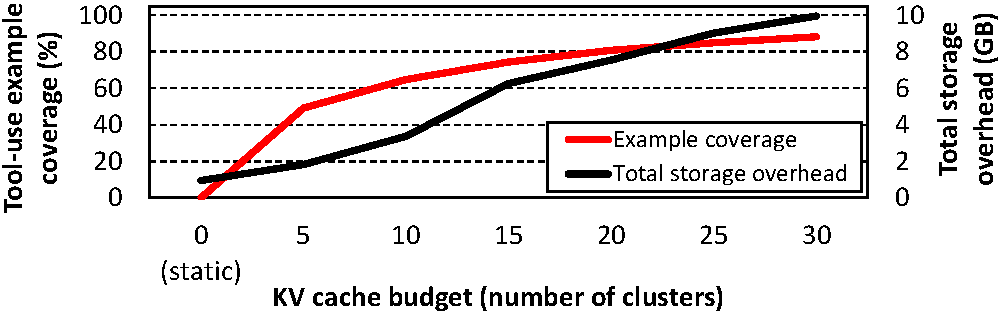
\includegraphics[width=\columnwidth]{./fig/eval_clustering}
\caption{
Tool-use example coverage (left, red) and total storage overhead (right, black) by KV cache budget.
}
\Description{Tool-use example coverage and total storage overhead by KV cache budget.}
\label{fig:eval_clustering}
\end{figure}

{\bf Storage overhead.}
Precomputed KV caches are stored in SSD, and loaded to memory on demand to reduce online prefill compute. Because the agentic workloads display long prompt lengths, the size of the KV cache is also large. Expanding the cluster budget boosts tool-use example coverage (\sect{sect:proposed_prefill}) but also raises storage cost, as shown in \fig{fig:eval_clustering}. At budget 0, only static tokens are cached, using 0.95 GB (0.57 GB, Planner + 0.39 GB, Arbiter). Coverage grows with larger budgets but levels off beyond 15 clusters. We therefore fix the budget at 15 clusters for the remainder of the evaluation, using 6.26 GB of storage for 74.4\% coverage.


\begin{figure}[t!] \centering
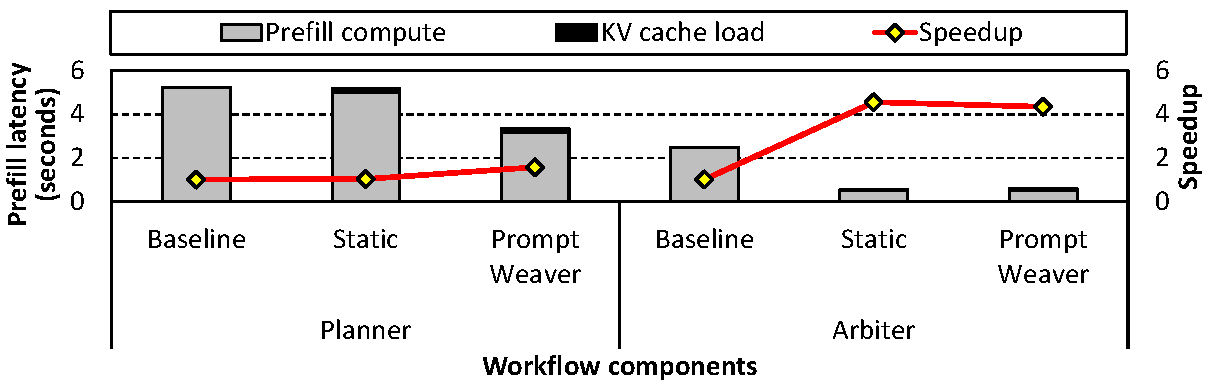
\includegraphics[width=\columnwidth]{./fig/eval_prefill_speedup}
\caption{
Prefill stage latency (left) and speedup gain (right) of \prefill.
}
\Description{Prefill stage latency and speedup gain of \prefill.}
\label{fig:eval_prefill_speedup}
\end{figure}

{\bf Speedup analysis.} 
\fig{fig:eval_prefill_speedup} quantifies impact of \prefill on Planner and Arbiter prefill stages. The Static design, caching only static tokens for the prompt, adds just a 1.01$\times$ speedup for Planner because while the amount of static tokens increases, the number of uncached dynamic tokens stays roughly the same (15.3\% decrease). In \prefill, clustered dynamic caching is applied on top of static token caching, achieving a 49.6\% reduction in the number of uncached input tokens and a 1.57$\times$ speedup. Meanwhile, \prefill reduces the amount of uncached input tokens by 88.9\% thanks to Arbiter's mostly static input tokens, achieving 4.35$\times$ speedup. Overall, loading KV cache from SSD storage adds minor overhead compared to the speedup achieved by compute savings, accounting for 5.8\% and 11.7\% of prefill latency in Planner and Arbiter, respectively.


\subsection{\decode} \label{sect:eval_decode}

{\bf Speedup analysis.}
\fig{fig:eval_decode_speedup} reports the decode stage latency of speculative decoding with draft LLM Llama-3.2-1B-Instruct~\cite{llama_3.2} (SpecDec) and \decode with a trigram ($n{=}3$) draft model. SpecDec experiences slowdown rather than speedup over the baseline. Other than the multi-token tax, the overhead that comes from dealing with different tokenizers between the target and the draft model~\cite{hf_uag} further slows down the system to achieve a much slower speed than was expected from \tab{tab:draft_specdec_accuracy}. On the contrary, the non-selective design of \decode effectively avoids any draft LLM-related overheads, speeding up the decode stage by 1.38$\times$. With selective decoding, \decode can avoid the multi-token tax when no draft tokens are accepted, falling back to autoregressive generation 17 (Planner) and 37 (Arbiter) times per query. Overall, \decode reduces the decode latency by 1.73$\times$, establishing itself as a lightweight and performant solution.


\begin{figure}[t!] \centering
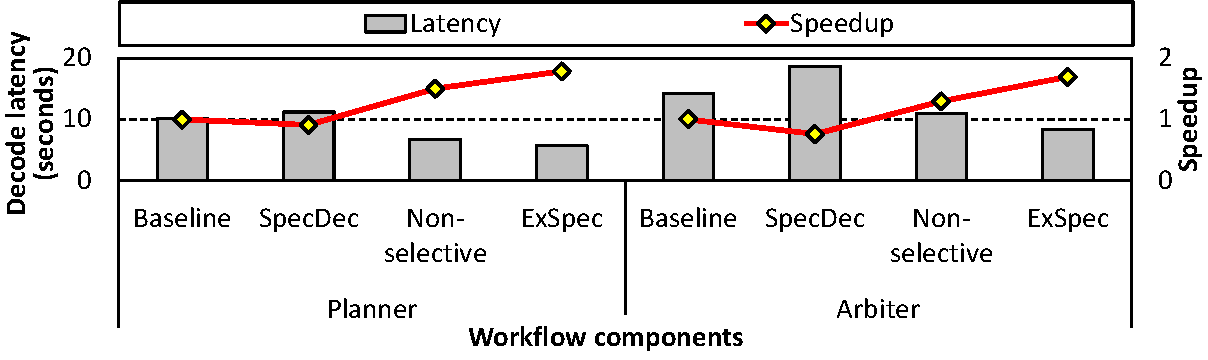
\includegraphics[width=\columnwidth]{./fig/eval_decode_speedup}
\caption{
Decode stage latency (left) and speedup (right) of speculative decoding (SpecDec) and \decode.
}
\Description{Decode stage latency and speedup of speculative decoding (SpecDec) and \decode.}
\label{fig:eval_decode_speedup}
\end{figure}


{\bf Draft token accuracy.}
\tab{tab:eval_draft_token_accuracy} compares draft-token accuracy under selective and non-selective \decode. Although non-selective decoding produces many more draft tokens, both modes accept the same number, underscoring the value of reverting to autoregressive generation when acceptance chances are low. Selective decoding thus increases overall accuracy, falling back to autoregressive generation on average 17 (Planner) and 37 (Arbiter) times per query.

{\bf $\bm{n}$-gram model generation overhead.}
While the $n$-gram model incurs constant-time latency per lookup, building the LUT takes $O(N)$ time for input token length $N$. The LUT generation takes up 83 milliseconds per query, indicating that it incurs a negligible overhead in terms of latency.


\subsection{\proposed Full System Integration} \label{sect:eval_end_to_end}

{\bf End-to-end speedup.}
\fig{fig:eval_end_to_end_speedup} shows the latency and speedup of end-to-end on-device agentic workloads. The impacts of \prefill (PW), \decode (ES), and \proposed (PW+ES) are shown. Applying \prefill and \decode independently provides end-to-end speedups of 1.16$\times$ and 1.43$\times$, respectively. Applying \prefill and \decode together reaps an end-to-end speedup of 1.61$\times$. Alongside the speedup, it is worth noting that \proposed is a purely software solution that can be directly applied to existing on-device agentic systems without degrading the accuracy of the agent.


\begin{table}[t]
\centering
\caption{
Draft token accuracy comparison between non-selective and selective decoding schemes of \decode.
}
\footnotesize
\resizebox{1.0\columnwidth}{!}{
\begin{tabular}{|c|c|c|c|c|}
\hline
\makecell[c]{\textbf{Workflow}\\ \textbf{component}} & \makecell[c]{\textbf{Applied}\\ \textbf{method}} & \makecell[c]{\textbf{Generated}\\ \textbf{draft tokens}} & \makecell[c]{\textbf{Accepted}\\ \textbf{draft tokens}} & \makecell[c]{\textbf{Draft token}\\ \textbf{accuracy}} \\
\hline
\multirow{2}{*}{\centering Planner} & Non-selective & 364 & 48 & 0.13 \\
\cline{2-5}
 & Selective & 194 & 48 & 0.25 \\
\hline
\multirow{2}{*}{\centering Arbiter} & Non-selective & 622 & 56 & 0.09 \\
\cline{2-5}
 & Selective & 218 &56 & 0.26 \\
\hline
\end{tabular}
}
\label{tab:eval_draft_token_accuracy}
\end{table}


\begin{figure}[t!] \centering
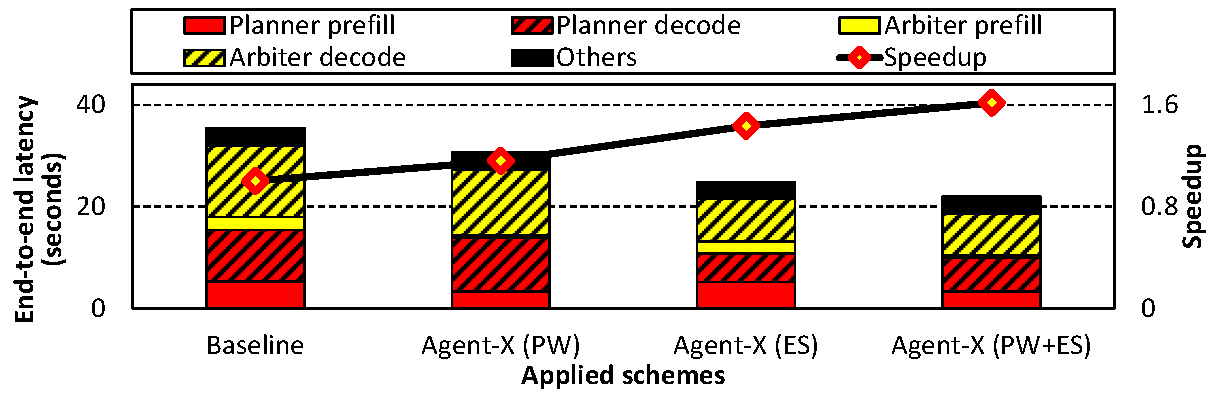
\includegraphics[width=\columnwidth]{./fig/eval_end_to_end_speedup}
\caption{
End-to-end latency (left) and speedup (right) of \proposed. PW denotes \prefill, ES denotes \decode, and PW+ES denotes the full \proposed pipeline.
}
\Description{End-to-end latency and speedup of \proposed.}
\label{fig:eval_end_to_end_speedup}
\end{figure}


\subsection{Discussions} \label{sect:eval_discussions}

{\bf Application to other platforms, agents, and models.}
As \prefill and \decode are both purely software solutions, \proposed can easily be ported to other hardware platforms. While our prototype is implemented on macOS due to the maturity of its local LLM ecosystem (TinyAgent), the core algorithms of \proposed are hardware-agnostic and applicable to other platforms. Because the fine-tuned model and datasets provided by TinyAgent are available only in macOS environments, an end-to-end evaluation of \proposed on other hardware platforms is challenging. We also evaluate \proposed on the smaller model TinyAgent-1.1B. \prefill and \decode achieve speedups of $1.62\times$ (prefill) and $1.42\times$ (decode), confirming their efficacy on smaller LLMs.

{\bf Fine-tuned models as draft LLM.}
We explore using TinyAgent-1.1B, fine-tuned for agentic tasks, as the draft model in applying speculative decoding to target TinyAgent-7B. Our experiments under the same setting as \fig{fig:eval_decode_speedup} show it is 1.81$\times$ slower than the baseline. Its draft token accuracy displays high variance across tasks, exhibiting unstable latency. Based on the TinyAgent paper~\cite{tinyagent}, we estimate its fine-tuning cost as 5 ExaFLOPs ($5\times10^{18}$ FLOPs), and even at 100\% compute utilization, it would take 75 hours to fine-tune TinyAgent-1.1B on our evaluation platform. Overall, the added fine-tuning cost and the resulting latency slowdown demonstrate that using a fine-tuned draft LLM is not beneficial, underscoring the effectiveness of \decode.

{\bf Robustness to tool-use distribution drift.}
To assess the effect of tool-use pattern drifts on \prefill, we evaluate a case where notes-related tools, namely \texttt{create\_note}, \texttt{open\_note}, and \texttt{append\_note\_content}, are disabled. \prefill only experiences a small accuracy drop (0.8\%p) and maintains high tool-use example coverage with 75.7\% at cache budget of 15 clusters. Overall, these numbers are close to those reported in \fig{fig:planner_accuracy_tokens} and \fig{fig:eval_clustering}, demonstrating the robustness of \prefill.

{\bf Effect of lengthened input prompt on decode latency.}
\prefill increases the average input tokens from 1,739 to 3,790 to enable prefix caching. This translates to an additional 256 MB of memory for the KV cache, forcing the memory bandwidth-bound decode stage to load more data. Consequently, the normalized decode stage latency, quantified as \emph{Time-Per-Output-Token}, increases by 2.2\% (from 122 ms to 125 ms), consistent with a 1.7\% rise in overall memory usage. However, the prefill speedup outweighs this minor decode overhead. Furthermore, additional tokens only apply to the Planner, reducing its impact on the full system pipeline.


\begin{figure}[t!] \centering
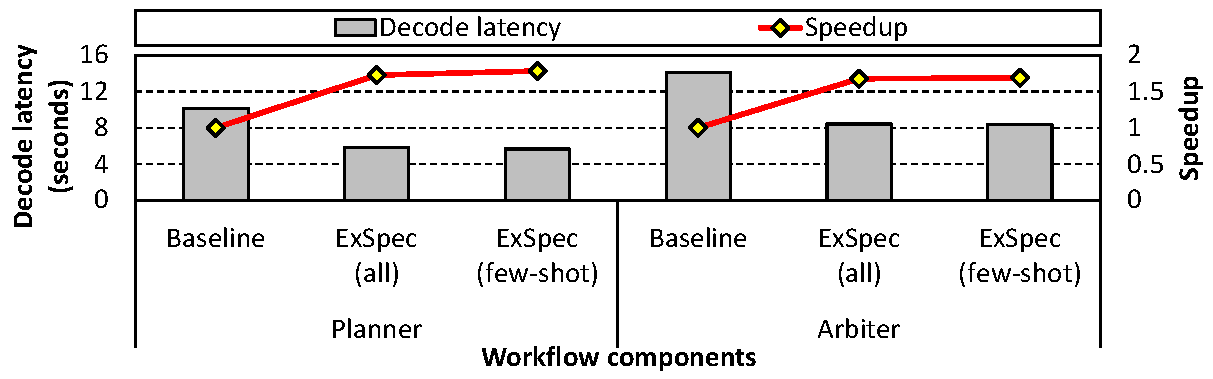
\includegraphics[width=\columnwidth]{./fig/discussion_extraction_region}
\caption{
Decode latency (left) and speedup (right) of \decode with varying extraction regions for LUT.
}
\Description{Decode latency and speedup of \decode with varying extraction regions for LUT.}
\label{fig:discussion_extraction_region}
\end{figure}


{\bf Prompt extraction region.}
\decode constructs the $n$-gram LUT using a portion of the input. To study the effect of the extraction region, we compare two cases: \decode~(all), which uses the entire input, and \decode~(few-shot), our proposed method, which extracts the few-shot examples and the user query. As shown in \fig{fig:discussion_extraction_region}, \decode~(all) still achieves a solid 1.70$\times$ speedup over the baseline. However, \decode~(few-shot) delivers an additional 3\% and 1\% speedup over \decode~(all) for the Planner and Arbiter, respectively. This indicates that the Planner is more sensitive to the choice of extraction region than the Arbiter. We attribute this sensitivity to the input size, where the Planner is 2.20$\times$ larger than Arbiter, therefore ``polluting'' the LUT with excess tokens.


{\bf Various \texorpdfstring{$n$}{n}-gram draft models.}
We examine how $n$ in \decode's $n$-gram model affects its effectiveness. A bigram model ($n{=}2$) causes the draft token accuracy to drop sharply to 0.10, a significant decrease compared to the default ($n{=}3$), which achieves 0.25. This result highlights the importance of the context length ($n{-}1$) in our $n$-gram draft model in generating accurate predictions. A quadgram model ($n{=}4$) further improves accuracy to 0.31, but produces only 72\% as many draft tokens as the trigram model. This reduction in the quadgram model stems from its longer context. A longer context makes \decode more conservative when generating draft tokens and increases the likelihood of falling back to autoregressive generation. Therefore, while a longer context increases accuracy, it reduces the number of draft tokens, ultimately leading to a 5.1\% slower total decode latency compared to the trigram model.



